\section*{Problema 3.1}

\textbf{Trabajamos con los de datos fashion MNIST. Se trata de imágenes 28x28 de diez diferentes tipos de prendas. Trabajaremos con \file{fashion-mnist\_train.csv}.  Ver \url{https://www.kaggle.com/zalando-research/fashionmnist}}

\begin{figure}[H]
    \centering
    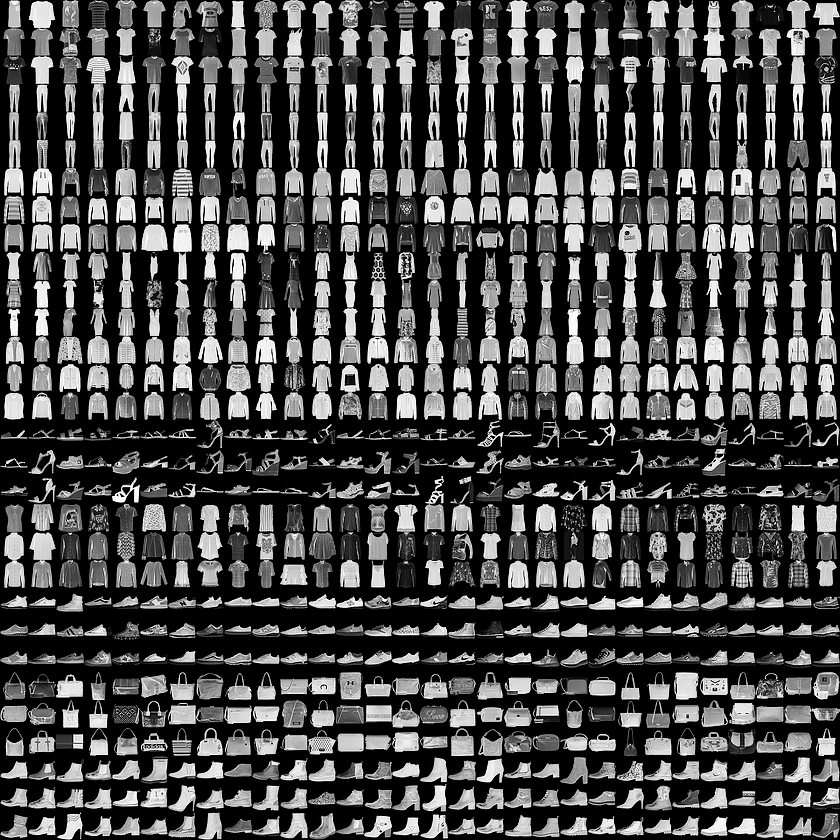
\includegraphics[width=8cm]{Graphics/Problema_3_1.png}
    \caption{Conjunto de datos contenido en el archivo \file{fashion-mnist\_train.csv}.}
\end{figure}

\textbf{Busca visualizaciones 2D y 3D basadas en PCA de las imágenes de T-shirts (clase "0`'). ¿ Ves posible encontrar interpretaciones de los componentes como lo hicimos en clase con la base mnist (clásico) de dígitos?}


\subsection*{Visualizaciones 2D}

En la figura \ref{fig:problema5_pca_2d} se visualzan las posiciones de las primeras dos componentes de PCA al ser aplicad a los datos del archivo \file{fashion-mnist\_train.csv}.
Se seleccionaron nueve camisetas que se encontraran lo más próximo a cada extremo del conjunto de la figura \ref{fig:problema5_pca_2d_camisetas}. Este conjunto se encuentra representado en la figura \ref{fig:problema5_pca_2d}. Las posiciones de las primeras dos componentes de PCA correspondientes de este subconjunto se muestran en la tabla \ref{table:pca_2d}.

\begin{figure}[H]
    \centering
    \begin{subfigure}{9.5cm}
        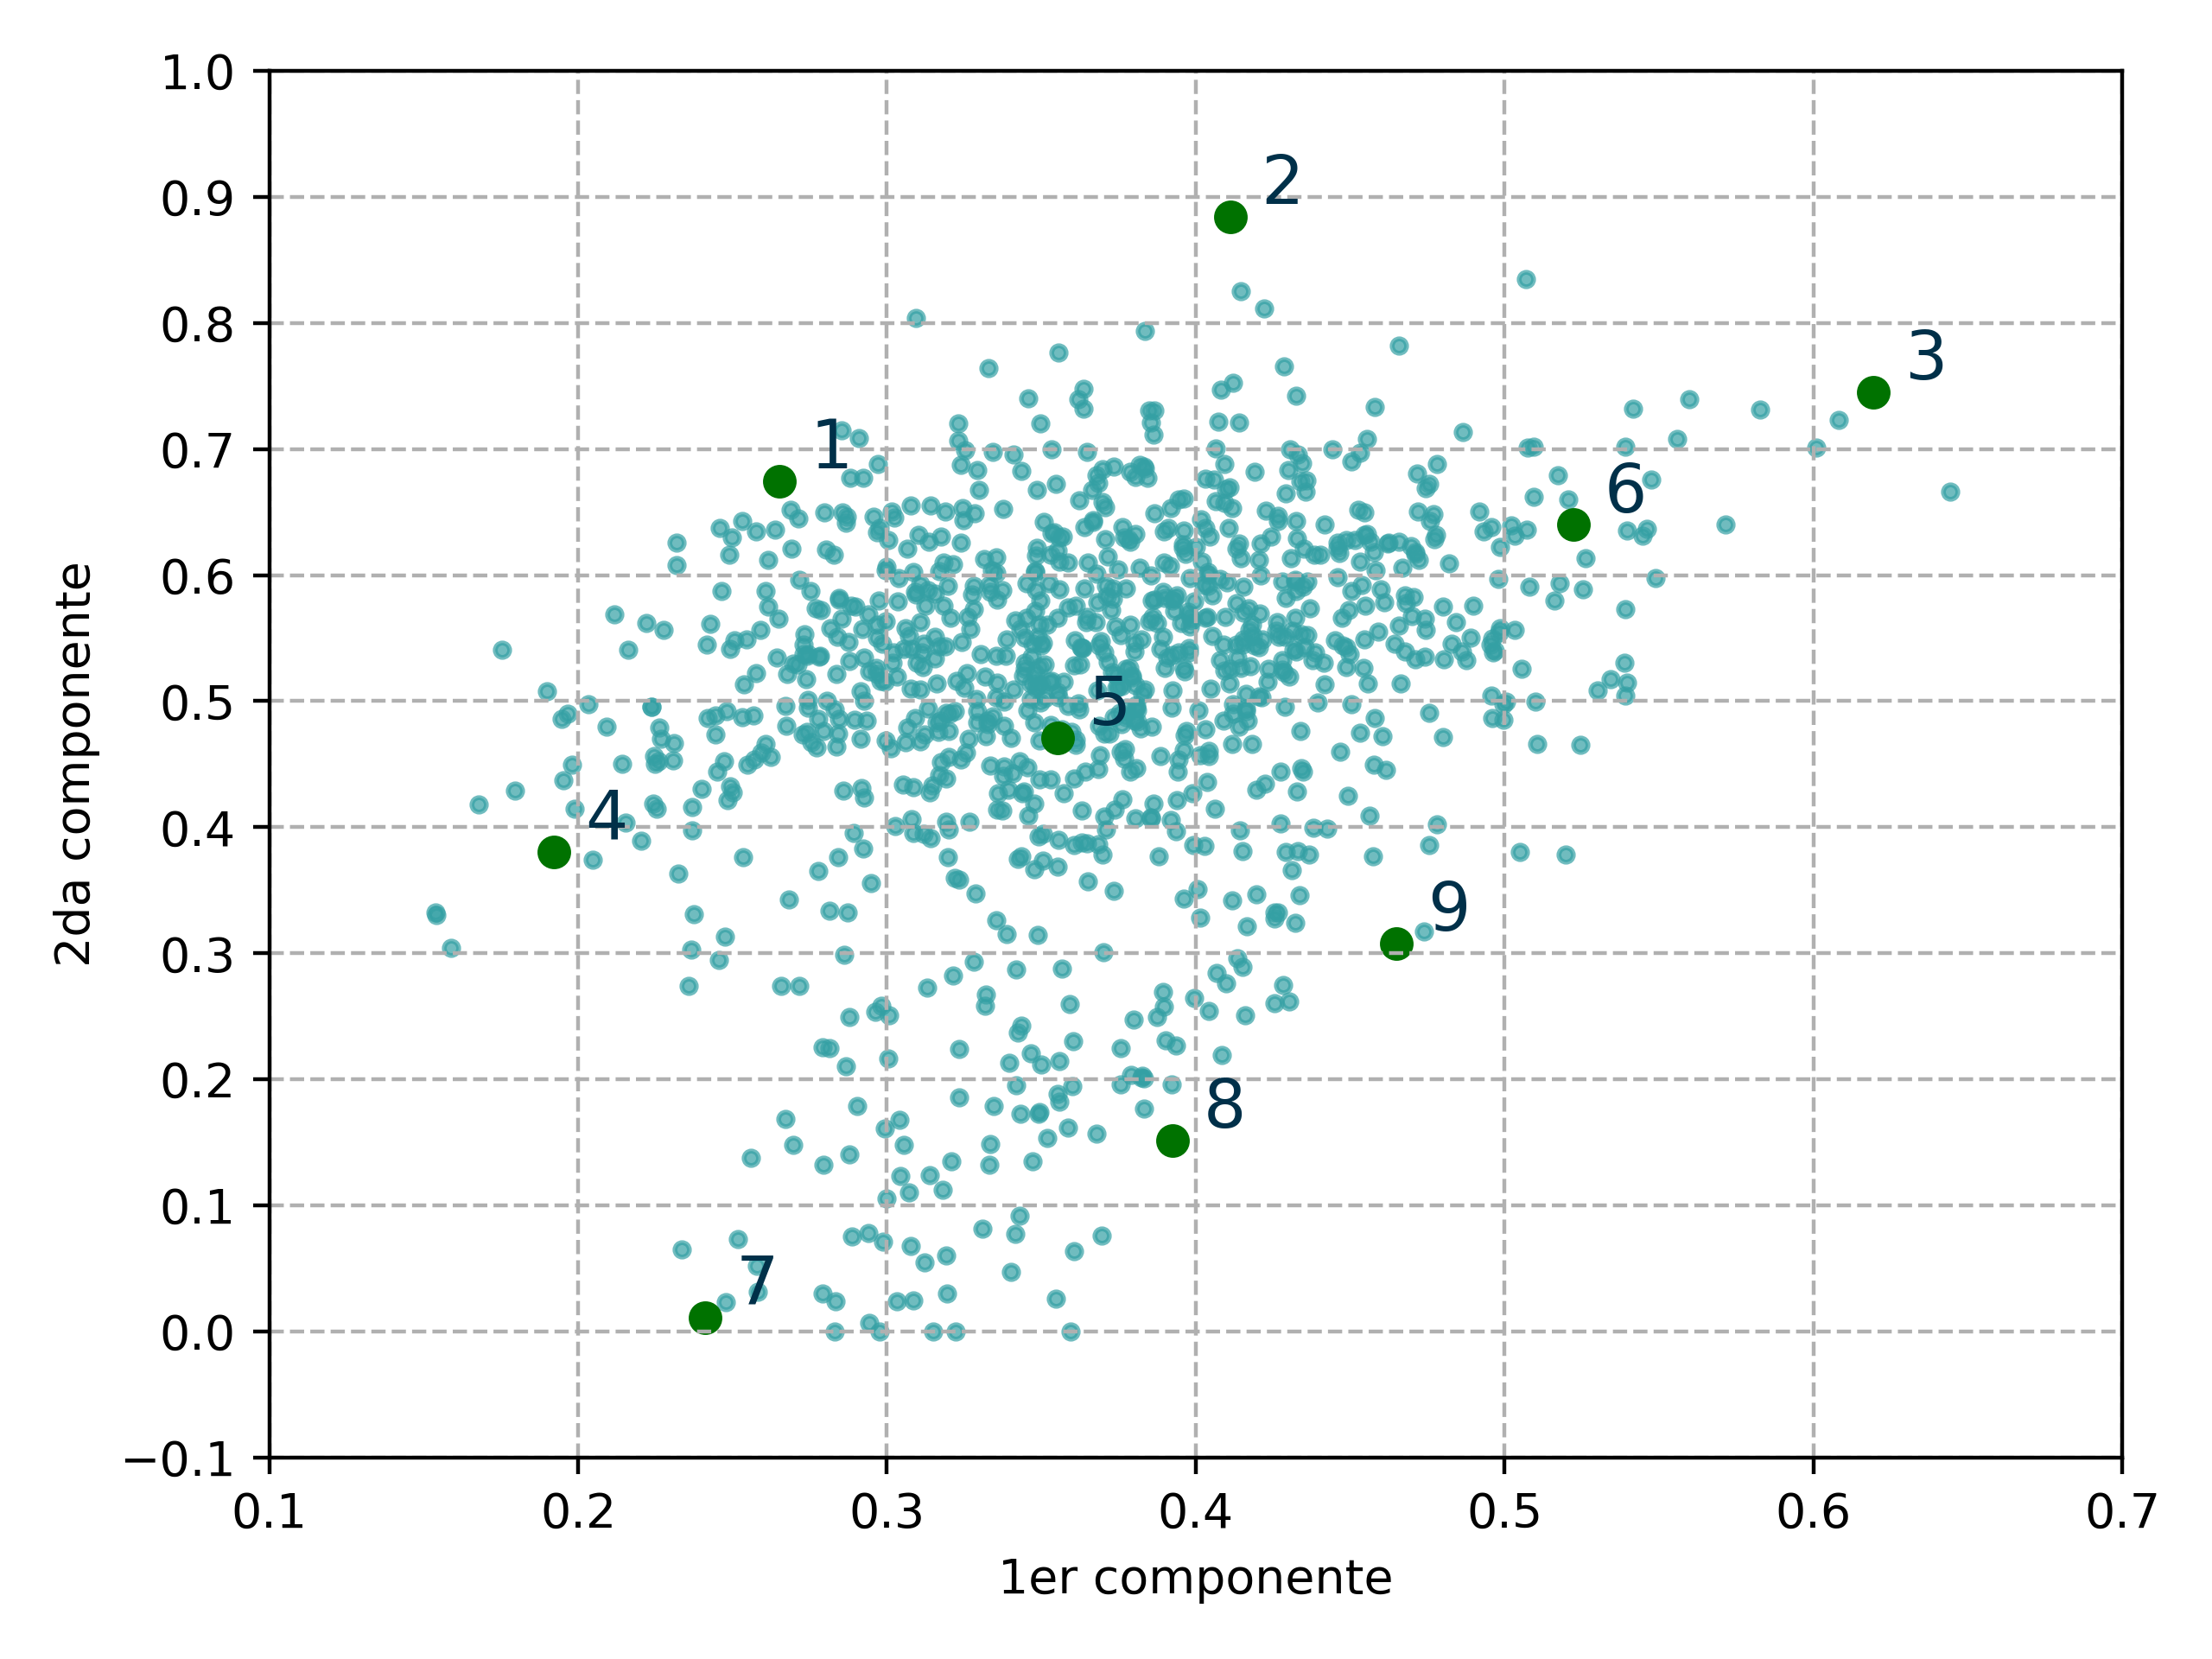
\includegraphics[width=9.5cm]{Graphics/Problema_3_1/loadings_2d.png}
        \caption{Resultados de PCA usando dos componentes.}
        \label{fig:problema5_pca_2d}
    \end{subfigure}
    \begin{subfigure}{7cm}
        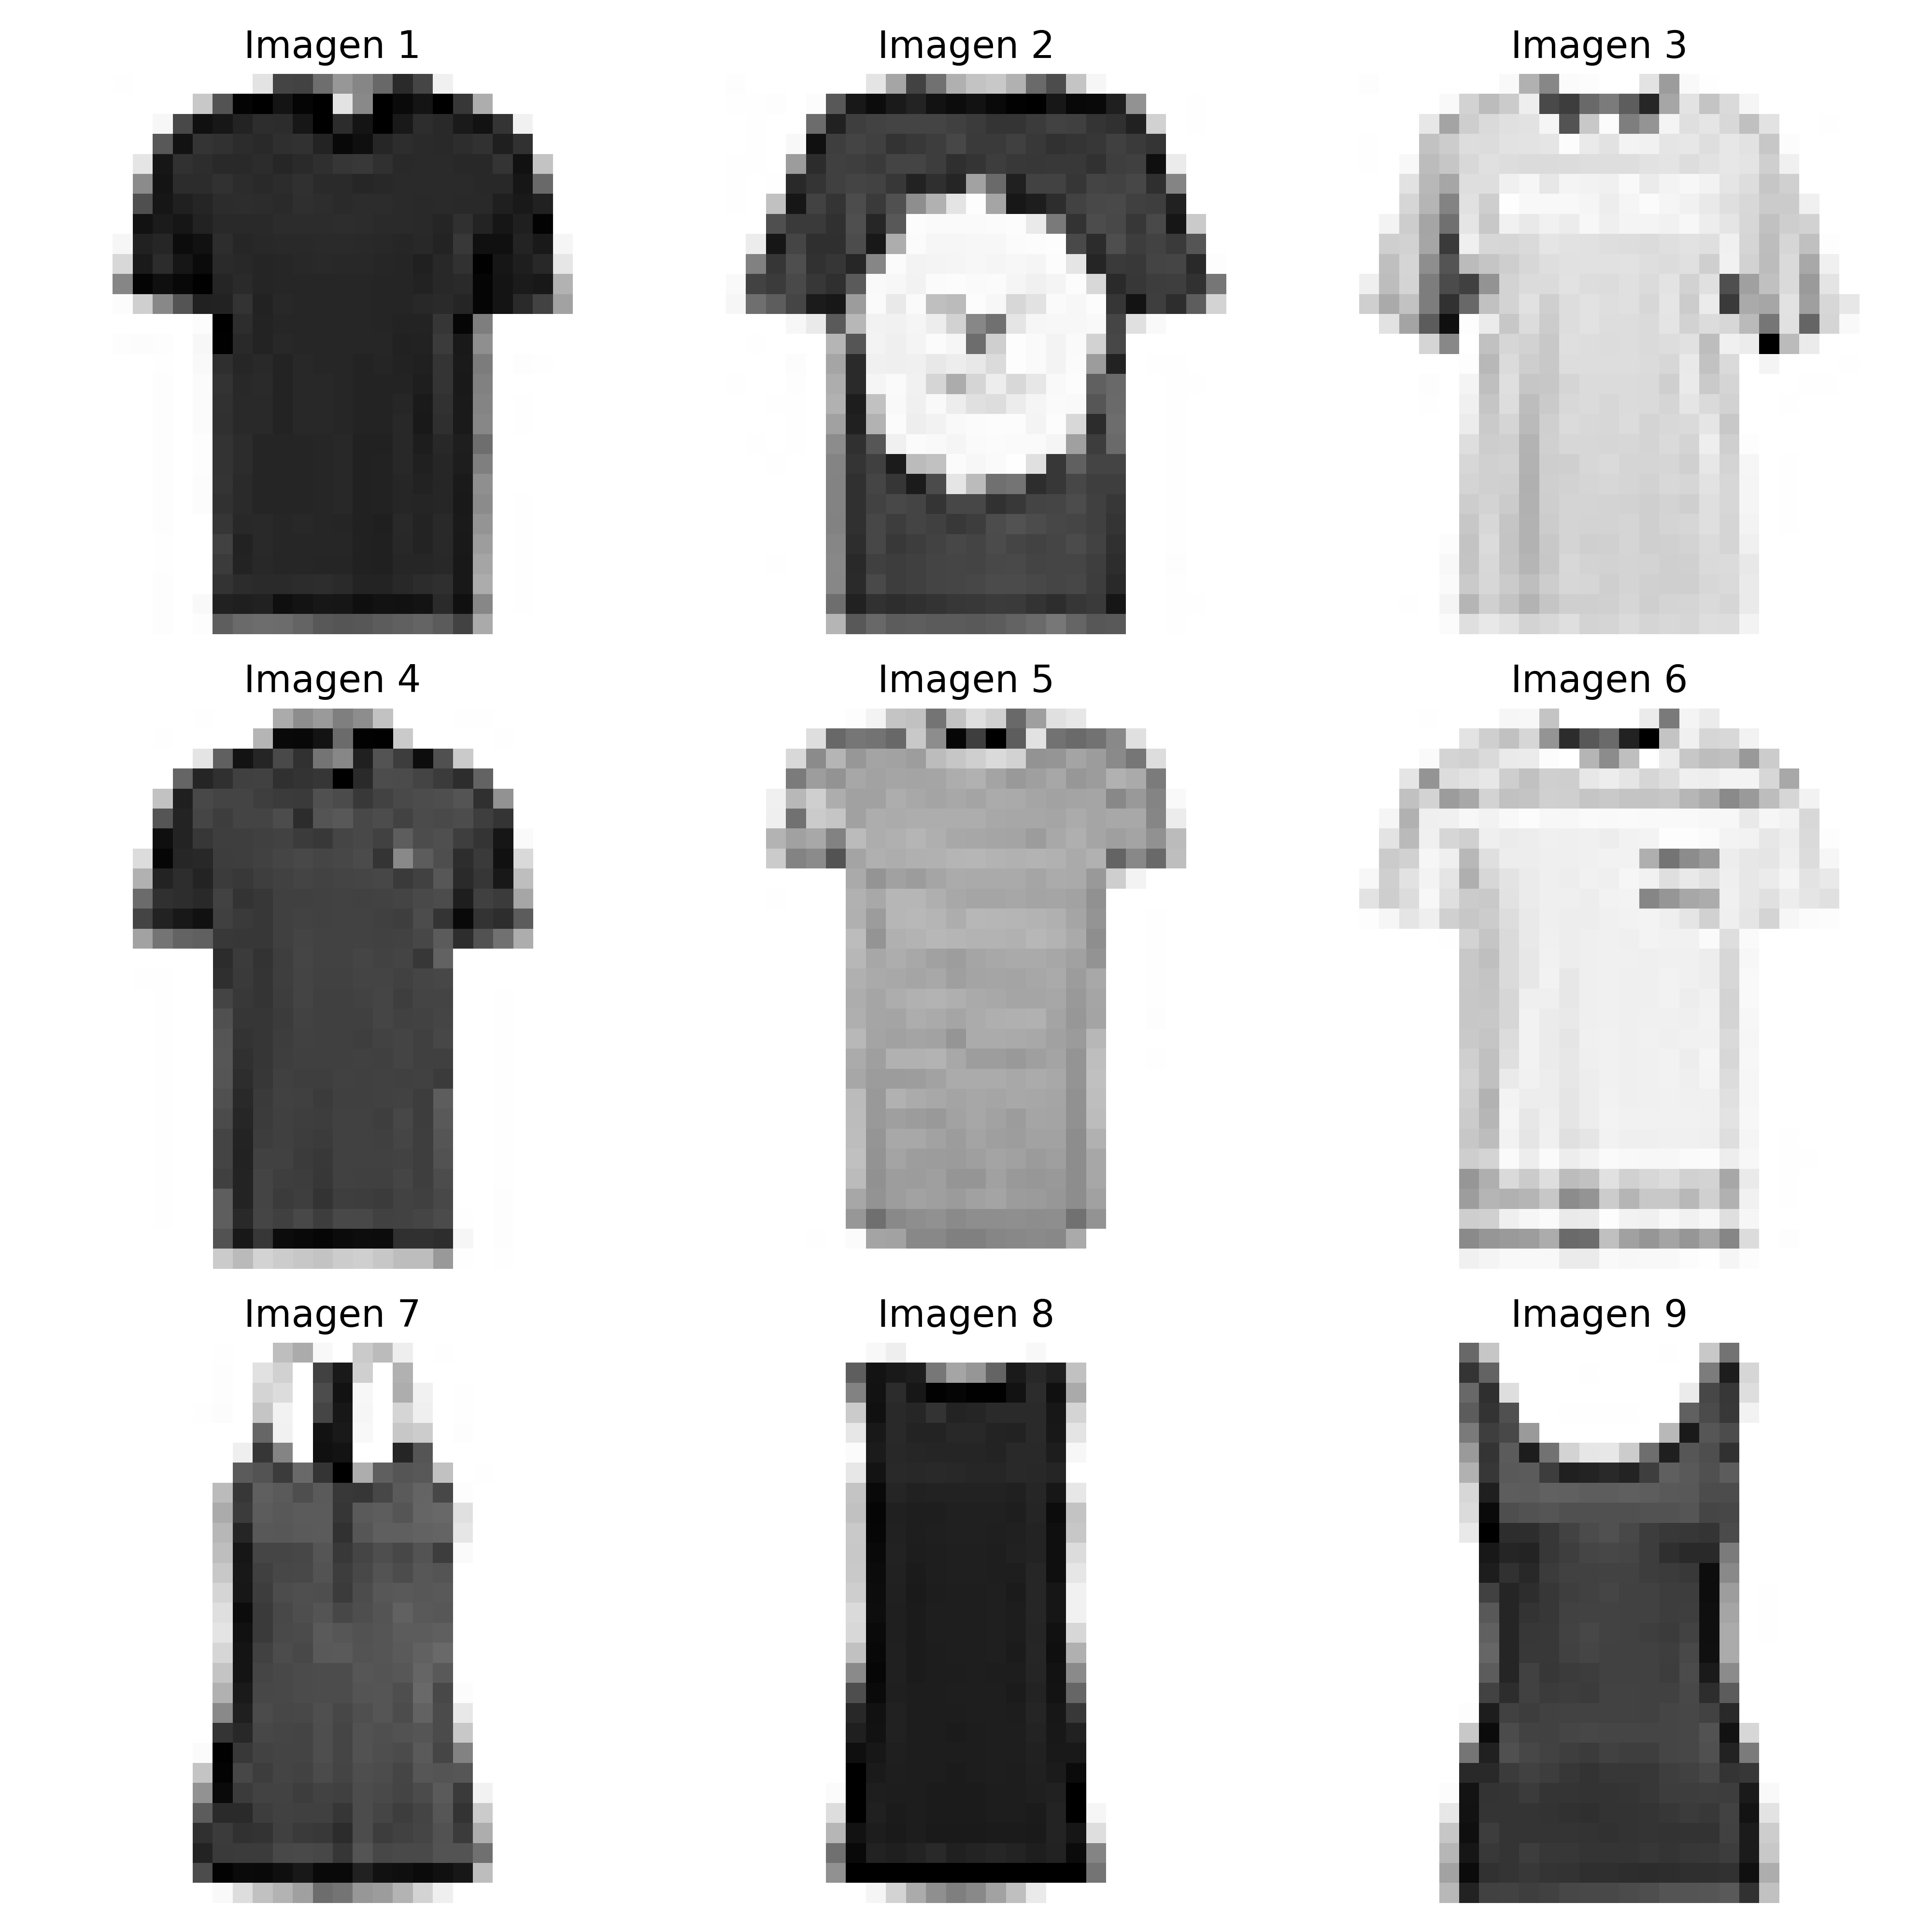
\includegraphics[width=7cm]{Graphics/Problema_3_1/T_shirts_2d.png}
        \caption{Camisetas señaladas en la figura \ref{fig:problema5_pca_2d}.}
        \label{fig:problema5_pca_2d_camisetas}
    \end{subfigure}
    \caption{Resultados de las primeras dos componentes de PCA para el conjunto de datos contenido en \file{fashion-mnist\_train.csv}.}
    \label{fig:pca_2d}
\end{figure}

\begin{table}[H]
    \centering
    \begin{tabular}{ccc} \hline
        \multirow{2}{*}{Imagen} & \multicolumn{2}{c}{Componente}          \\
                                & 1                              & 2      \\ \hline
        1                       & 0.2652                         & 0.6747 \\
        2                       & 0.4111                         & 0.8843 \\
        3                       & 0.6193                         & 0.7453 \\
        4                       & 0.1923                         & 0.3806 \\
        5                       & 0.3552                         & 0.471  \\
        6                       & 0.5223                         & 0.64   \\
        7                       & 0.241                          & 0.011  \\
        8                       & 0.3925                         & 0.1517 \\
        9                       & 0.465                          & 0.3078 \\ \hline
    \end{tabular}
    \caption{Resultados numéricos de las primeras dos componentes de PCA usando el subconjunto señalado en la figura \ref{fig:problema5_pca_2d_camisetas}.}
    \label{table:pca_2d}
\end{table}

Realizando una búsqueda en los patrones encotrados se encuentran los siguientes:

\begin{itemize}
    \item Para la primer componente de PCA pudo hacer una separación entre las camisetas de color oscuro en la parte izquierda y conforme se avanza hacia la derecha las camisetas toman un color más claro.
    \item Para la segunda componente de PCA se pudo encontrar que las camisetas que se encuentran en la parte inferior contienen una nula o muy poca cantidad de información en el cuello. En la parte intermedia se encuentran camisetas con cuello más marcado y en la parte supeior camisetas con cuello delgado.
\end{itemize}

\subsection*{Visualizaciones 3D}

Usando las primeras tres componentes de PCA se obtuvieron los resulados mostrados en la figura \ref{fig:problema5_pca_3d}. Se seleccionaron camisetas que se encontraran en la parte inferior, intermedia y superior usando unicamente la tercer componente. El subconjunto de las camisetas seleccionadas se encuentra representado en la figura \ref{fig:problema5_pca_3d_camisetas}. Los valores numéricos de las primeras tres componentes de PCA de las camisetas selecionadas se encuentran en la tabla \ref{table:pca_3d}.

\begin{figure}[H]
    \centering
    \begin{subfigure}{8.5cm}
        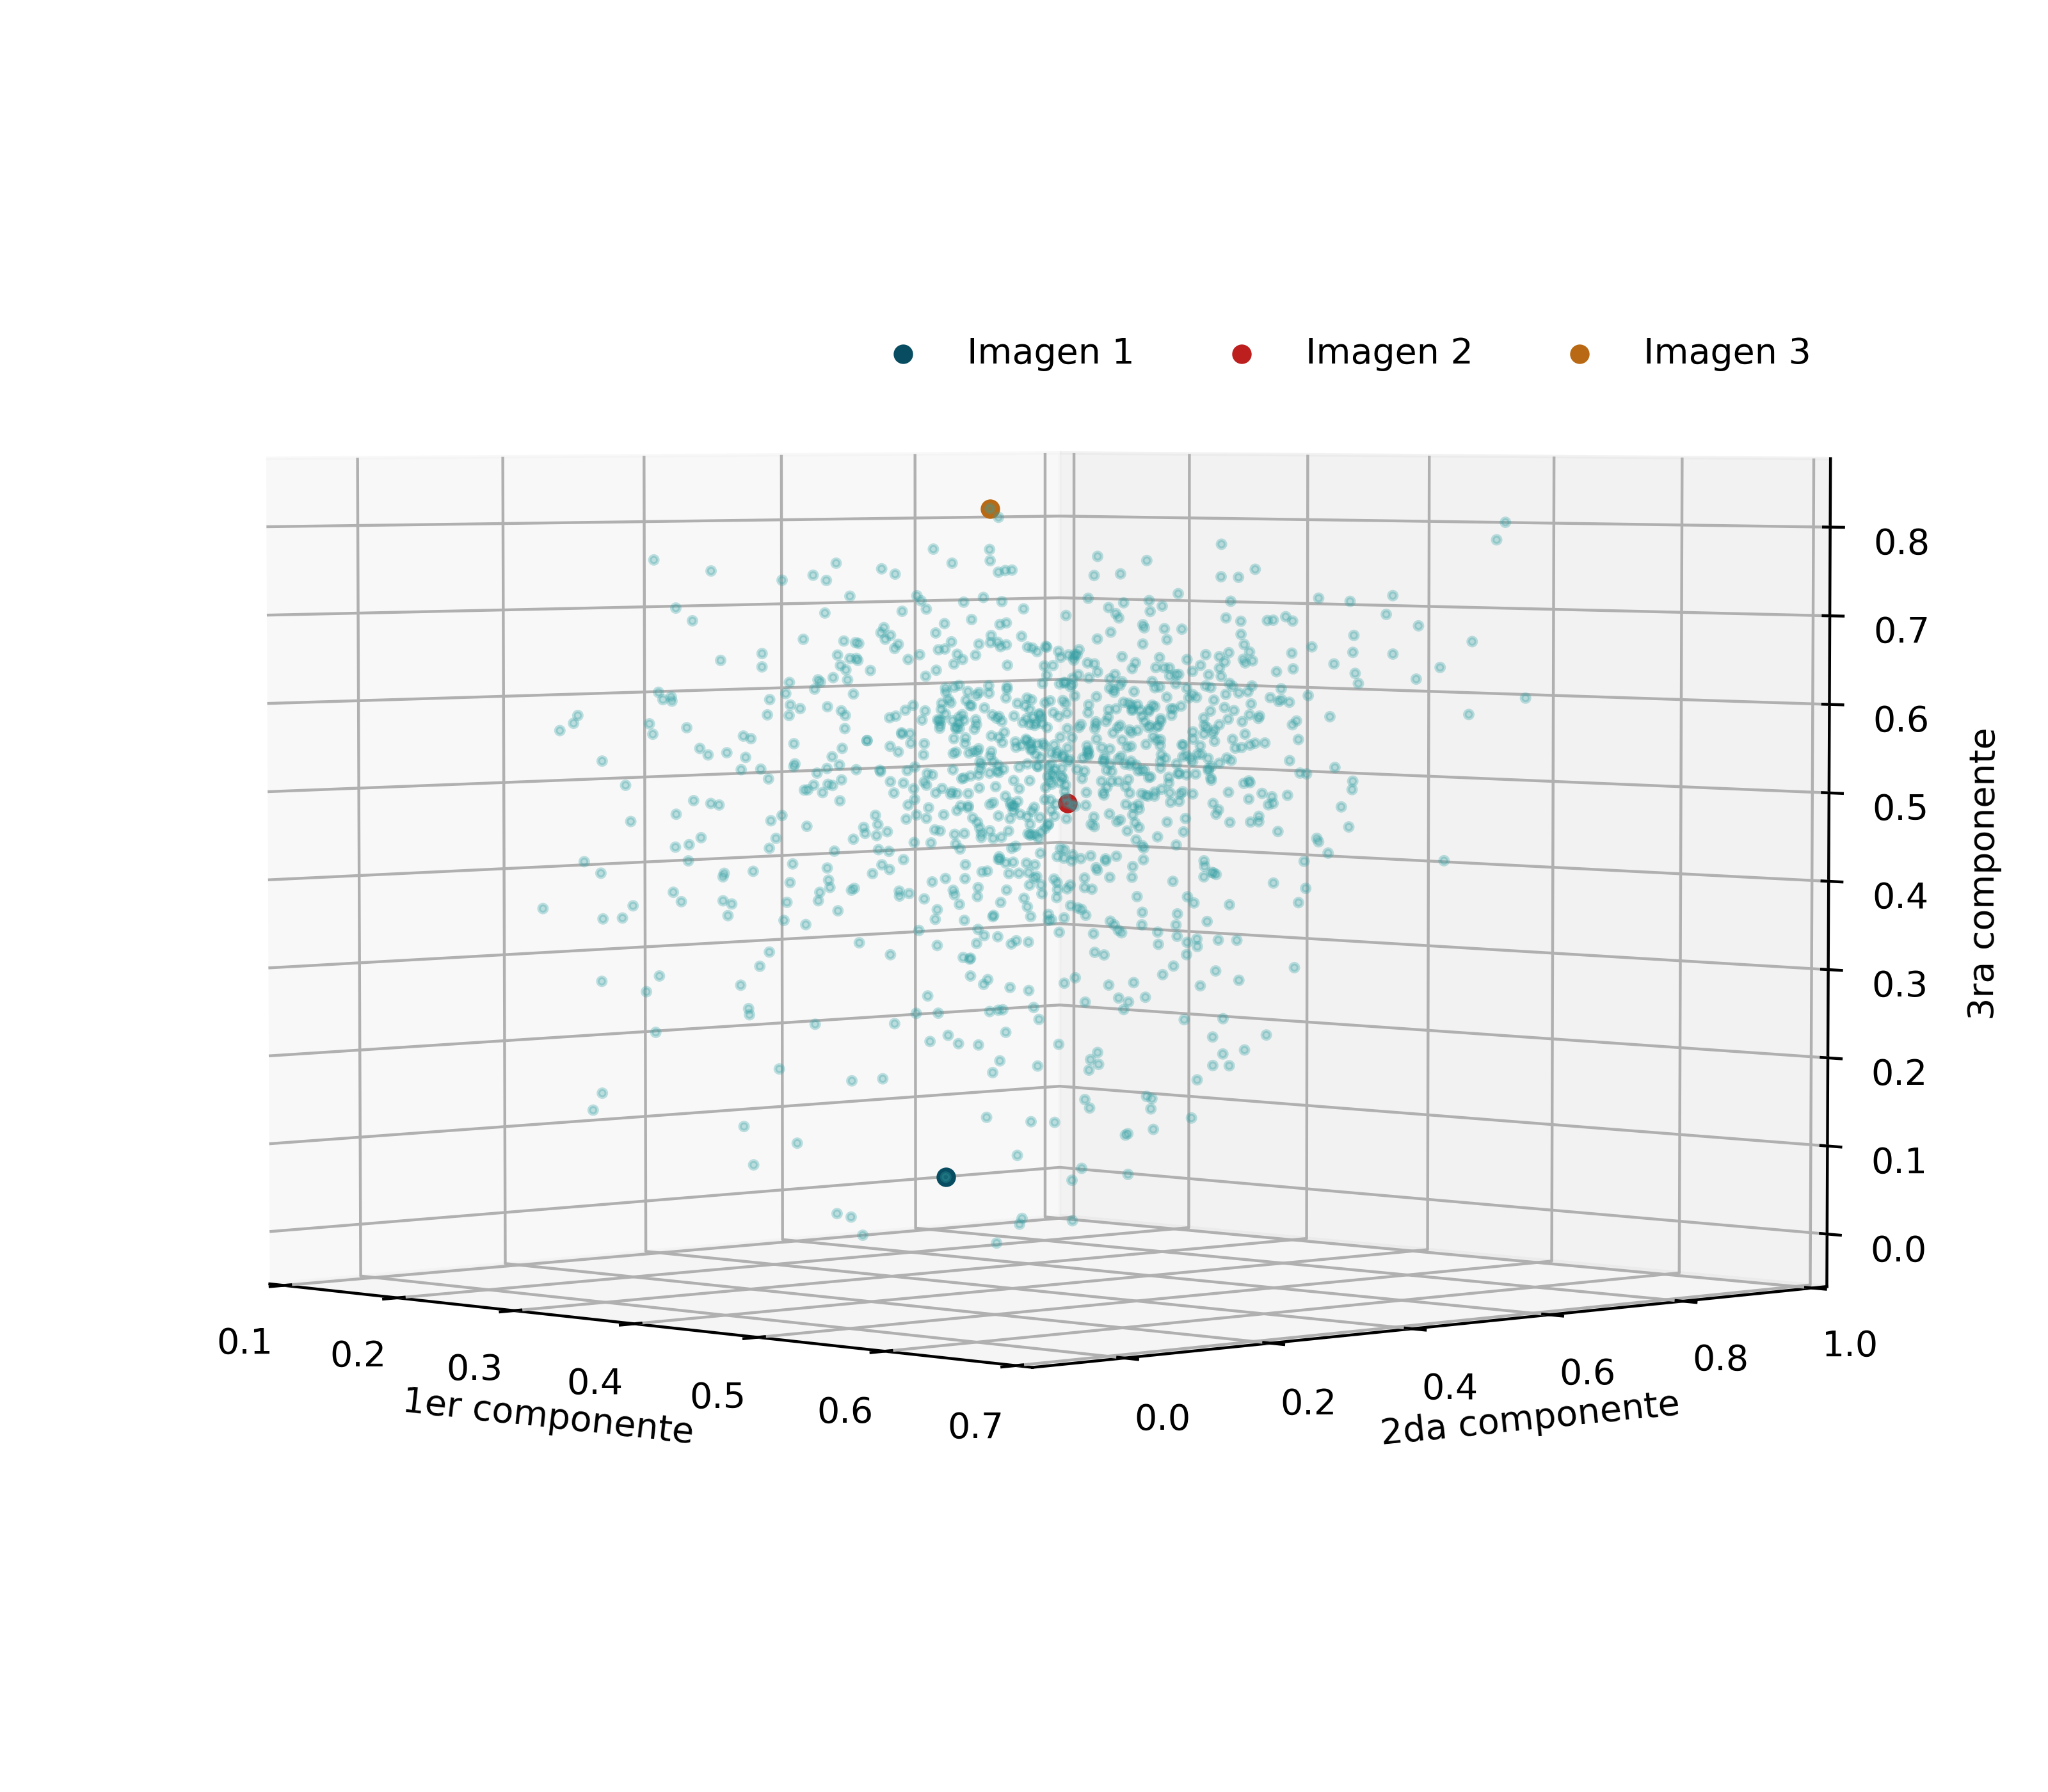
\includegraphics[width=8.5cm]{Graphics/Problema_3_1/loadings_3d.png}
        \caption{Resultados de PCA usando dos componentes.}
        \label{fig:problema5_pca_3d}
    \end{subfigure}
    \begin{subfigure}{8cm}
        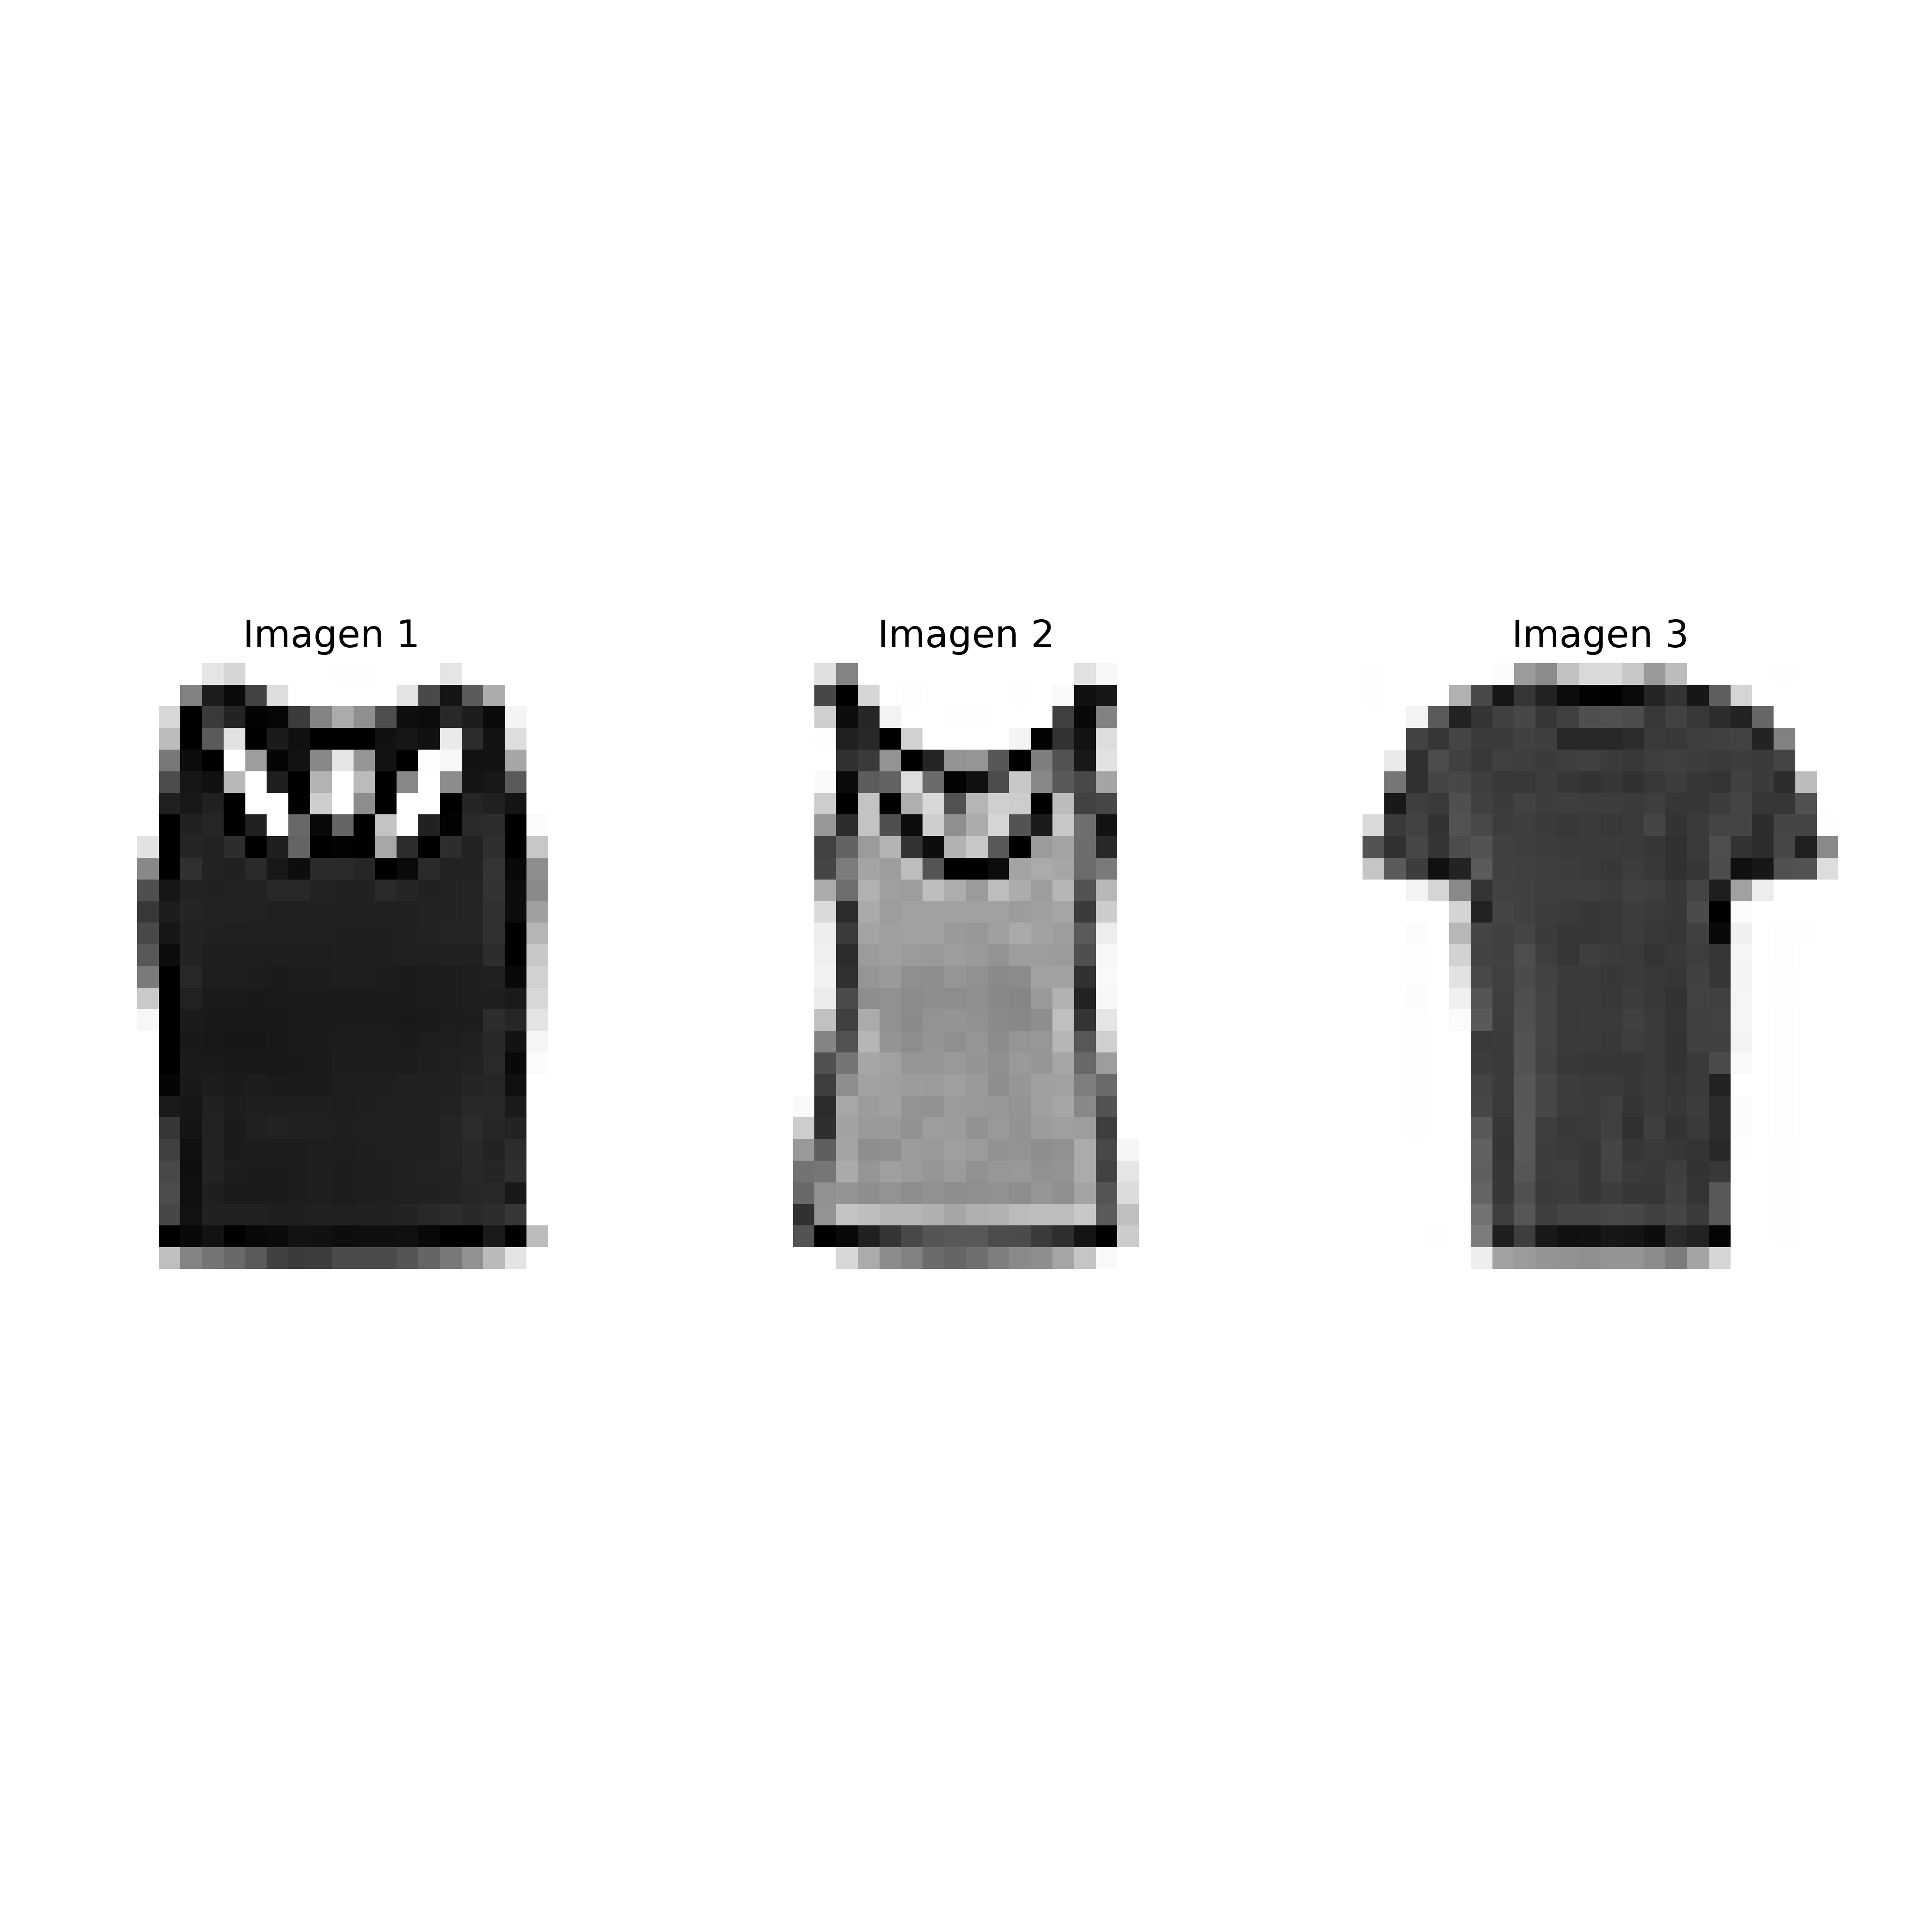
\includegraphics[width=8cm]{Graphics/Problema_3_1/T_shirts_3d.png}
        \caption{Camisetas señaladas en la figura \ref{fig:problema5_pca_3d}.}
        \label{fig:problema5_pca_3d_camisetas}
    \end{subfigure}
    \caption{Resultados de las primeras tres componentes de PCA para el conjunto de datos contenido en \file{fashion-mnist\_train.csv}.}
    \label{fig:pca_3d}
\end{figure}

\begin{table}[H]
    \centering
    \begin{tabular}{cccc} \hline
        \multirow{2}{*}{Imagen} & \multicolumn{3}{c}{Componente}                   \\
                                & 1                              & 2      & 3      \\ \hline
        1                       & 0.3374                         & 0.4134 & 0.058  \\
        2                       & 0.4574                         & 0.377  & 0.494  \\
        3                       & 0.292                          & 0.5571 & 0.8176 \\ \hline
    \end{tabular}
    \caption{Resultados numéricos de las primeras tres componentes de PCA usando el subconjunto señalado en la figura \ref{fig:problema5_pca_3d_camisetas}.}
    \label{table:pca_3d}
\end{table}

La intepretación que se le puede dar a la tercer componente de PCA es la siguiente:

\begin{itemize}
    \item Las camisetas que se encuentren en la parte inferior contienen una cantidad nula de mangas. Las camisetas que se encuentren en la parte intemedia presentan un crecimiento en la parte superior de la camiseta. En la parte superior se encuentran camisetas con mangas.
\end{itemize}